\section{Physical geometry of Afghanistan}
\begin{figure}[!ht]
  \centering
  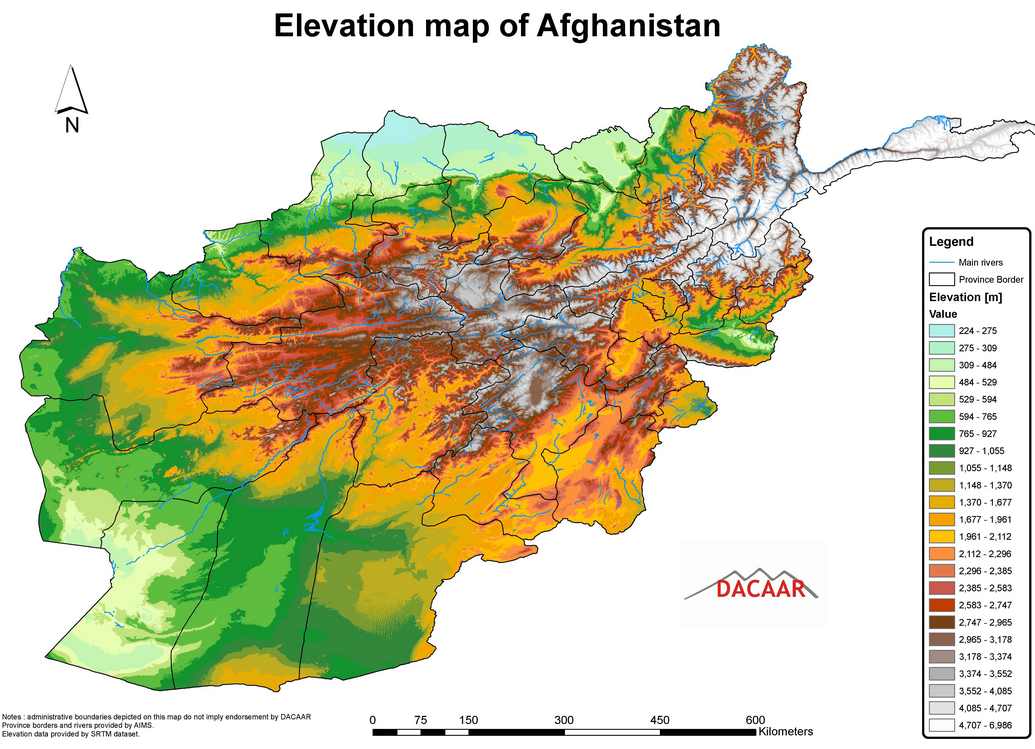
\includegraphics[width=10cm]{00 - Images/afghan-topography.png}
  \caption{Elevation Map Of Afghanistan \cite{afghan-topo}}
  \label{fig:af_elev}
\end{figure}

When discussing robot locomotion, it is important to analyze the threats that the physical geography might pose to the logistic tasks that the robot has to do, with a focus on the country with the highest amount of casualties due to landmines, more specifically Afghanistan figure \ref{fig:af_elev} shows that from northeast to southwest the Hindu kush mountains divide Afghanistan into three regions 

\begin{enumerate}
    \item The central highlands spans $\frac{2}{3}$ of the country (Mountainous and rugged terrain) 
    
    \vspace{-4mm}
    
    \item The southwestern plateau spans $\frac{1}{4}$ of the country (Arid region, desert, and semi-desert)
    
    \vspace{-4mm}
    
    \item The smaller northern plains (Fertile soil)
\end{enumerate}

The mountains from the central highlands stretch into the southwestern plateau and the northern plains, meaning that logistics in Afghanistan troublesome the robot will be facing either mountainous terrain, arid terrain, or fertile land, all three being rugged due to the large number of mountains stretching throughout the country. \cite{ellicott2003junior}

\subsubsection*{Weather}

The climate of Afghanistan tends to be just as rough as the terrain, it tends to range from light annual rainfall to almost no annual rainfall, the central highlands (subarctic climate) can reach temperatures as low as -26\textdegree C and as high as 53\textdegree C. In the southwestern plateau and northern plains, the temperature ranges between -8\textdegree C and 46\textdegree C 

\vspace{2mm}

Between June and September, strong winds tend to blow, and those can have a velocity up to 180km/h and rainfall is sparse, but can happen during the winter period. During the winter period, rainfall tends to be snow in the central highlands. \cite{ellicott2003junior}


